\documentclass[12pt]{jarticle} 
%\documentstyle[12pt,fleqn,epsf,iepaper,cite]{jarticle}
%\documentstyle[12pt,iepaper,eclepsf,oddchar]{jarticle}
\usepackage[dvipdfm]{graphicx}
\usepackage{iepaper}
\usepackage{epsf}
\usepackage{ccaption}
\usepackage{algorithm}
\usepackage{algorithmic}
\usepackage{subcaption}
\usepackage{enumerate}
\usepackage{comment}
\usepackage{url}
\usepackage{multirow}
\usepackage{diagbox}
\usepackage{amssymb}
\usepackage{mathtools}
\usepackage{wrapfig}
\usepackage{graphicx}
\usepackage{float}
\usepackage{amsmath}
\usepackage{lipsum}
\usepackage[jis2004]{otf}

\title{深層強化学習に基づく
\par
トレーディングカードゲーム環境の構築}
\author{西村 昭賢} 
\gakuseki{1201201100}[B]  %卒論はB,修論はM
\group{第 1 研究グループ}            % 卒論の場合
\shidou{森 直樹 教授}                          % 卒論の場合
%\syusa{教授}                            % 修論の場合
%\hukusa{教授}{教授}

%図番号を「(section番号).(図番号)」とするため
\makeatletter
 \renewcommand{\thefigure}{%
   \thesection.\arabic{figure}}
  \@addtoreset{figure}{section}
\makeatother

\makeatletter
 \renewcommand{\thetable}{%
   \thesection.\arabic{table}}
  \@addtoreset{table}{section}
\makeatother

\makeatletter
 \renewcommand{\theequation}{%
   \thesection.\arabic{equation}}
  \@addtoreset{equation}{section}
\makeatother


\begin{document} 
\maketitle 
\pagenumbering{roman} 
%%% 目次
\tableofcontents
\newpage
%
%% 図一覧
\listoffigures
\newpage 

%% 表一覧
 \listoftables
 \newpage

\pagenumbering{arabic} 

% 文書開始
\newpage
\changeindent{0cm}
\section{はじめに}
\changeindent{2cm}

近年, 人工知能に関する研究分野は目覚ましい発展を遂げており様々な分野に応用されている. その中でも人間の学習プロセスに近いとされる強化学習と深層学習を融合した深層強化学習は自動運転やロボット, 推薦システム等の実生活の問題解決への応用例が数多く報告されている \cite{Vehicle}\cite{robotics}\cite{recommendation}. 
実世界の問題解決への応用だけでなく, 深層強化学習はゲームへの応用も盛んである.
特に将棋や囲碁といった, プレイヤーが意思決定をする段階でそれ以前の意思決定の過程がすべて把握可能な完全情報ゲームへの応用においては AlphaGo \cite{AlphaGo}, AlphaZero \cite{AlphaZero} を筆頭に現役のプロプレイヤーを圧倒する性能を残しており成果が顕著である. 
最近では麻雀やポーカーのような, プレイヤーに与えられる情報が部分的である不完全情報ゲームへの応用も注目されている.
\par
本研究では不完全情報ゲームであるトレーディングカードゲーム環境への深層強化学習の適用と深層強化学習を用いたゲームバランス調整手法を提案し, 独自に構築したトレーディングカードゲーム環境を用いて数値実験することでその有効性を示す. 
\par
以下に本論文の構成を示す.  まず, 2 章では本研究で用いる要素技術について, 3 章では類似研究と提案手法について説明する. 4 章では本環境で独自に構築したトレーディングカードゲーム環境の概要を示す. 5 章で実験方法の説明をし, 6 章で実験結果と考察を示す. そして, 7 章に本研究のまとめ及び今後の課題について述べる.
\clearpage

\section{要素技術}

\subsection{OpenAI Gym}
OpenAI Gym \cite{OpenAIGym} は非営利企業 OpenAI が提供する強化学習のシミュレーション用ライブラリであり, 強化学習の環境として図 \ref{fig:OpenAIGymSample} に示すように多くのゲーム, シミュレータが登録されている. さらには提供されているインターフェースに沿って, エージェントの行動空間や状態空間, 報酬などを定義,実装することで自作の強化学習環境を構築し利用することができる. 様々な強化学習用ライブラリに対応しているため比較的容易に強化学習を試すことができる.

\begin{figure}[ht]
  \centering
  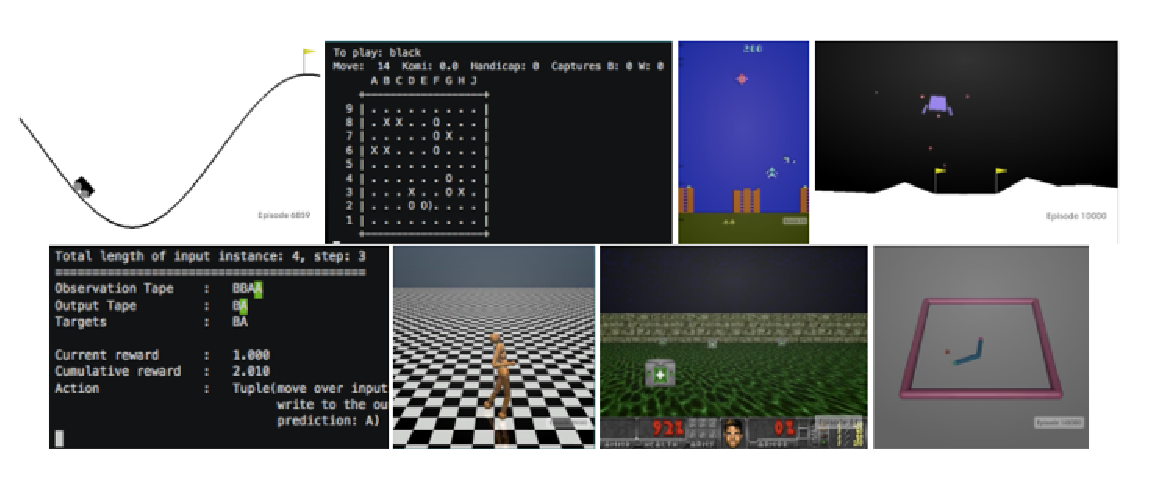
\includegraphics[width=150mm]{assets/OpenAiGym.eps}
  \caption{OpenAI Gym が提供している様々な環境}
  \label{fig:OpenAIGymSample}
\end{figure}



\subsection{Q 学習}
強化学習では,エージェントが行動することで環境における状態が変化し報酬を得る. 強化学習における行動はその直後に獲得する報酬の大きさではなく, 未来に渡っての報酬の総和を見積もった値である「価値」の最大化に繋がるかという観点で評価される.
価値の最大化を目指す場合にはある状態 $s$ において行動 $a$ をとった時の価値が分かればよい.この価値のことを Q 値, あるいは行動価値関数と呼ぶ. この Q 値を基に行動を選択していく価値ベースの強化学習手法において代表的な手法が Q 学習である. 
 Q 学習ではエージェントの 1 ステップごとに (\ref{updateQ}) 式に示す更新式で Q 値を更新する.
\begin{equation}
  \centering
  \label{updateQ}
  Q(s_t,a_t) \leftarrow Q(s_t,a_t) + 
   \alpha(r_{t+1} + \gamma \mathrm{max}_{a_{t+1}}Q(s_{t+1},a_{t+1}) - Q(s_t,a_t))
\end{equation}
なお $t$ は時間, $r$ は報酬, $\alpha$ は Q 値の更新度合いを表す学習率, $\gamma$ は将来の価値の割引度合いを表す割引率である. 
\par
また, Q 学習に代表される強化学習においては環境の調査を目的とする探索と, 探索により得られた良い報酬を得ることができる経験の活用をそれぞれどの程度にすればよいかといういわゆる「探索と活用のトレードオフ」という問題が発生する. これを解決する手法として一般的なものが $\mathrm{\epsilon - greedy}$ 法である. $\mathrm{\epsilon - greedy}$ 法では確率 $\epsilon$ でランダムに行動し探索, それ以外では経験を活用して価値が最も高い行動を選択することで探索と活用のバランスをとっている.  


\subsection{Deep Q Network}
Q 学習を実際に実装する場合, 状態と行動をインデックスとした Q 値のテーブルを作成する. しかし状態空間や行動空間が高次元である, あるいは状態や行動が離散値ではなく連続値で表現される場合には Q テーブルのメモリ量は爆発してしまう. この問題を解決した技術が Deep Q Network (DQN) \cite{DQN} である.
 DQN ではニューラルネットワークを用いて, ある状態における行動ごとの Q 値を推定することでたとえ状態が連続値であっても学習可能としている. DQN では, エージェントが経験した過去の体験を Replay Memory に一定期間保存しておき, 過去の経験をランダムにサンプリングして学習する Experience Replay や行動を決定する Q 値のネットワークと Q 値を学習するネットワークを分けることで Q 値の過大評価を防ぐ Fixed Target Network といった工夫により安定した学習を可能としている.

 \begin{figure}[H]
  \begin{algorithm}[H]
      \caption{
        deep Q-learning with experience replay
        }
      \label{alg1}
      \begin{algorithmic}[1] 
      \STATE Initialize replay memory $D$ to capacity $N$
      \STATE Initialize action-value function $Q$ with random weights $\theta$
      \STATE Initialize target action-value function $\hat{Q}$ with weights $\theta^{-}$ = $\theta$
      \FOR{episode = 1, $M$} 
      \STATE Initialize sequence $s_{1} = \{x_1\}$ and preprocessed sequence $\phi_1$ = $\phi(s_1)$ 
      \FOR{$t$ = 1, $T$}
      \STATE With probability $\epsilon$ select a random action $a_{t}$
      \STATE otherwise select $a_t = \mathrm{argmax}_{a}Q(\phi(s_{t}),a; \theta)$
      \STATE Execute action $a_t$ in emulator and observe reward $r_t$ and image $x_{t+1}$
      \STATE Set $s_{t+1} = s_t,a_t,x_{t+1} and preprocess \phi{t+1} = \phi(s_{t+1}) $
      \STATE Store transition $(\phi_t,a_t,r_t,\phi_{t+1})$ in $D$
      \STATE Sample random minibatch of transitions $(\phi_j,a_j,r_j,w_{j+1})$ from $D$
      \STATE 
      \begin{equation*} 
        \mathrm{Set} y_j = 
        \left\{
          \begin{aligned}
              r_j \quad & \text{if episode terminates at step } j + 1 \\
              r_j + \gamma \mathrm{max}_{a'} \hat{Q}(\phi_{j+1},a';\theta^{-}) \quad  & \text{otherwise}\\
          \end{aligned}
        \right.     
      \end{equation*}      
      \STATE Perform a gradient descent step on $(y_j - Q(\phi_j,a_j;\theta))^2$ with respect to the network parameters $\theta$
      \STATE Every C steps reset $\hat{Q} = Q$
        
      \ENDFOR
      \ENDFOR
      \end{algorithmic}
  \end{algorithm}
  \caption{DQN のアルゴリズムの疑似コード \cite{DQN_algorithm}}
  \end{figure}

\subsection{Genetic Algorithm}
Genetic Alogorithm (GA) とは, 生物の進化と進化の過程を模した最適化手法であり, 主に組み合わせ最適化問題に対して適用される. GA では 1 つの解を 1 つの個体として表現し, 多数の個体からなる個体群を用いて解空間の多点を同時に探索する. 各個体はどの程度良い解であるかという指標として適用度を持つ. また, 各個体は染色体と呼ばれる配列で表される. この染色体を構成する要素を遺伝子, 染色体上の遺伝子が収まる座標を遺伝子座と呼ぶ. 探索においては, 個体群に対して選択, 交叉, 突然変異と呼ばれる 3 種類の遺伝演算子を適用させ世代と呼ばれる探索ステップを進めていく.\par
選択では, 探索において適用度が良好な個体が存在する部分を重点化するように現在の個体群から個体を選び, 次世代の個体群を生成する. 選択方法としては, 個体の適応度に比例する確率で個体を選択するルーレット戦略, 個体群からランダムに数個個体を抽出しその中で最も良好な個体を選択するトーナメント戦略がある. またこれらと併用される戦略として各世代の最良個体を保存するエリート保存戦略がある. エリート保存戦略により探索で発見した良い個体が失われることを防ぐことができる. 
交叉では, 2 つの個体からそれらの形質を受け継いだ新たな個体を生成する. 交叉においても染色体のランダムな 1 点で染色体を切断し部分列を染色体同士で交換する 1 点交叉, ランダムな 2 点で切断する 2 点交叉, 遺伝子座ごとランダムに交換する一様交叉など様々な方法がある. 
突然変異では, 各遺伝子座の遺伝子を許容された範囲の遺伝子の内容に置換する.
交叉や突然変異にはそれぞれ確率が設定されていることが一般的である. 



\subsection{Nondominated
Sorting Genetic Algorithm II}
Nondominated
Sorting Genetic Algorithm II (NSGA-II) とは, 

\clearpage
\section{提案手法}
本研究では, トレーディングカードゲーム環境を作成し環境におけるデッキ間の勝率を最適化した. 最適化の過程において深層強化学習と GA を組み合わせて, 調整するカードの枚数を最小化するような最適化手法を提案する.

\subsection{トレーディングカードゲーム環境}
本研究において構築した環境は, Magic : The Gathering \footnote[1]{https://magic.wizards.com} に代表されるトレーディングカードゲーム (Trading Card Game : TCG) を参考にした. TCG は 2 人のプレイヤーからなるゲームである. 囲碁や将棋のように, プレイヤーは先攻と後攻に分かれてターン制で進行していく. TCG の大きな特徴として, 囲碁や将棋のように各プレイヤーが同じユニット群を持つのではなく事前に各プレイヤーの選択による異なるユニットからなるデッキを構築することが挙げられる. また, TCG はゲームタイトルごとに細かいルールは異なるが, 一般的に相手プレイヤーのカードの 1 部分はプレイヤーから観測できない不完全情報ゲームである. 
以下, 実装したカードゲームのルールと用語を説明する.
\subsubsection{プレイヤー}
一般的な TCG と同様に, ゲームは 2 人のプレイヤーからなり, プレイヤーは複数のカードからなるデッキを持つ. 
プレイヤーは手札, 盤面と呼ばれるカードを保有する領域を持ち, ドローと呼ばれる操作でカードをデッキから手札に加える. また, プレイと呼ばれる操作でカードを手札から盤面に出す. また, デッキからカードが無くなった状態をデッキ切れと呼ぶ.  
また, プレイヤー自身が HP, マナという 2 つの整数値パラメータを持つ.
プレイヤー自身の HP が 0 となればゲーム敗北となり, 相手のカードからの攻撃などで減少していく.
マナはカードをプレイする際, 後述するカードのコスト分減少する. プレイヤーは残りマナを超えるコストを持つカードをプレイすることができない. 
今回の環境ではプレイヤーの HP の最大値は 20, マナの上限値は初期値が 1 で最大値を 5 と設定した.
\subsubsection{カード}
カードはそれぞれ攻撃力と HP とコストの 3 つの整数値パラメータを持つ.  盤面にあるカードは対戦相手の盤面にあるカード, あるいは相手プレイヤーに攻撃することができる. カードが攻撃する際には, 相手盤面に存在する攻撃対象のカードの HP, あるいは相手プレイヤーの HP へとカードの持つ攻撃力分ダメージを与える. またカードへと攻撃する際には攻撃対象のカードが持つ攻撃力分, 攻撃するカードもダメージを受ける.
ただし, 攻撃が可能となるのはカードが盤面にプレイされたターンの次のターンからになる. 
カードの HP が 0 になった, あるいは後述する手札と盤面の枚数制限を超えて盤面にプレイされた時はカードは破壊される. 破壊されたカードはゲームから取り除かれる. 
また, カードによっては以下に示す特殊効果を持つものもある.

\begin{description}
  \item[召喚 :]  盤面に出したら (攻撃力 , HP) = (1 , 1) の
  ユニットを追加で盤面に出す
  \item[治癒 :]  盤面に出したら自プレイヤーの HP を 2 回復する
  \item[攻撃 :]  盤面に出したら敵プレイヤーの HP を 2 減らす
  \item[取得 :]  盤面に出したら自プレイヤーは 1 枚カードをドローする
  \item[速攻 :]  盤面に出たターンに攻撃できる
\end{description}

\subsubsection{ゲームフロー}
以下, ゲームの流れを説明する.
\begin{enumerate}
  \setlength{\itemsep}{0cm} % 項目間
  \item ゲーム開始時に各プレイヤーは自身のデッキをシャッフル.
  \item デッキから初期手札としてカードを 5 枚ドロー. 
  \item 先攻プレイヤーは 1 ターン目のドローステップをスキップし行動.
  \item 後攻プレイヤーはカードを 1 枚ドローして行動.
  \item 2 ターン目以降は先攻プレイヤーもカードを 1 枚ドローしてから行動. 
  \item 4 , 5 の繰り返し. なお, ターンプレイヤーは行動前にマナを上限値まで回復. このときマナの上限値が 5 でなければ上限値を 1 増やしてから回復.
  \item プレイヤーがデッキ切れになっている状態でカードをドローしようとした, あるいはプレイヤー自身の HP が 0 となった場合はそのプレイヤーが敗北となりゲーム終了.
\end{enumerate}
\par
本構築環境では一般的な TCG と同様にカードがプレイされた次のターンから行動可能となるため, 先攻プレイヤーがカードの行動が早くなり有利となる.そのため, 先攻の 1 ターン目のドローステップをスキップしている. 


\subsection{関連研究}
\label{hearthstone}
トレーディングカードゲーム環境におけるバランス調整に関して, Fernando らは HearthStone \footnote[2]{https://hearthstone.blizzard.com} 環境内においてデッキ間の勝率が 50 \% となるように, 3 つのデッキの計 64 枚のカードにおける 180 個の調整可能なパラメータを 180 個の要素を持つ 1 次元配列として GA, NSGA-II を適用した\cite{EvolvingHearthStone}.
GA を用いた場合, デッキ間の勝率をほぼ 50 \% に近づけるという目標は達成したが, 180 個の調整可能パラメータの総変更量は 402 となり元のデッキの原型が無くなった. 
NSGA-II において勝率とパラメータの総変更量の 2 つの目的関数を最適化するように設定した場合, 勝率は GA を用いた場合とほぼ変わらず, パラメータの総変更量は 402 から 154 へと減少した.
\par
しかし, NSGA-II を用いることで GA に比べてカードのパラメータの総変更量は減少したが, 変更を及ぼす領域は調整対象のカード全体に及んでいる.  
本研究における提案手法は, 遺伝的アルゴリズムの解空間の次元を深層強化学習によるシミュレーションを参考に削減することで, 調整を施すカードの数を減らすことを目的としている.

\subsection{提案手法 : 深層強化学習によるデッキ内のカードパワーの測定}
TCG において, デッキ内の各カードのカードパワーを測る指標としてはそのカードがプレイされたときの勝率 (Win Rate when Play : WRP) などが考えられる. しかし, カードにコストが存在する場合においては低コストのカードと高コストのカードについてプレイされる回数に偏りが生じてしまう. このため, 得られる結果はカードのコストの影響が反映されてしまい意味のある結果とはいえない. \par
本研究では, 同デッキ同戦略のプレイヤーを先攻後攻両方に配置してカードを 1 種類ずつデッキから除いた場合の勝率をデッキ内のすべてのカードについて計算することで戦略下におけるデッキ内のカードパワーを測定する手法を提案する. 

\subsection{提案手法 : GA における解空間の次元を削減した最適化}
新たにデッキをトレーディングカードゲーム環境へと追加する際, デッキ間の勝率は $50 \pm 5 \%$ になることが環境として好ましい. \ref{hearthstone} 節で述べたようにトレーディングカードゲーム環境におけるデッキ間の勝率の最適化において GA の有用性が知られている. 本研究では, 深層強化学習を用いたシミュレーションによってデッキ内のカードにおいて調整するべきかどうか優先順位を定義し, 変更するカードを明確にしたまま GA の解空間を削減したトレーディングカードゲーム環境の最適化手法を提案する. 

\clearpage
\section{実験方法}
\subsection{実験 1 : 深層強化学習によるエージェント構築}
構築したトレーディングカードゲーム環境へ深層強化学習を適用する. 
深層強化学習手法として DQN を用いて構築環境において後攻のプレイヤーとして学習し, 学習済のエージェントで 10000 回ゲームを実行して勝率を計算した. 
また, 学習が進み具合を把握するため学習時の獲得報酬の推移を記録した.
さらに学習済エージェントを用いて 50000 回の対戦を実行し,エージェントが選択した行動の総数, 各カードごとのプレイされた総数を記録し学習済エージェントがどのような戦略を構築したか, それが人間から見て合理的な戦略かどうか考察した.

\subsubsection{対戦相手の行動ルーチンと対応するデッキ}
学習時, また学習後の対戦は共通して同一の対戦相手を設定した. 
対戦相手の戦略として, TCG における代表的な戦略として挙げられるアグロとコントロールの 2 種類を設定した. アグロとコントロールは様々な解釈がありデッキのカードの構成として定義されることもあるが, 本研究では以下のようにカードの攻撃の際の戦略として定義する. 詳細な疑似コードは, 

\begin{description}
  \item[アグロ :]  敵プレイヤーへの攻撃を優先しなるべく早くゲームエンドに持ち込む. 
  \item[コントロール :]  相手の盤面のカードの処理を優先し, 長期戦に持ち込む.
\end{description}

\begin{figure}[ht]
  \vspace{-0.3cm}
  \begin{algorithm}[H]
    \small
      \caption{
        対戦相手の行動ルーチン (アグロ)
        }
      \label{alg_aggro}
      \begin{algorithmic}[1] 
      \STATE 手札から盤面にカードを出せるだけプレイ (ドロー順が古い方から)
      \FOR{自盤面のカード (プレイ順が古い方から)}
      \IF{敵の盤面にカードが無い}
      \STATE 敵プレイヤーを攻撃
      \ELSE
      \IF{自身の HP が 12 以上}
      \STATE 敵プレイヤーを攻撃
      \ELSE
      \IF{敵盤面に破壊できるカードがある}
      \STATE そのカードを攻撃
      \ELSE
      \STATE 敵プレイヤーを攻撃
      \ENDIF
      \ENDIF
      \ENDIF
      \ENDFOR
      \STATE ターンを終了
      \end{algorithmic}
  \end{algorithm}
  \caption{アグロの疑似コード}
  \end{figure}

  \begin{figure}[ht]
    \vspace{-0.3cm}
    \begin{algorithm}[H]
      \small
        \caption{
          対戦相手の行動ルーチン (コントロール)
          }
        \label{alg_controll}
        \begin{algorithmic}[1] 
        \STATE 手札から盤面にカードを出せるだけプレイ (ドロー順が古い方から)
        \FOR{自盤面のカード (プレイ順が古い方から)}
        \IF{敵の盤面にカードが無い}
        \STATE 敵プレイヤーを攻撃
        \ELSE
        \IF{自盤面の行動可能なカード全てで敵プレイヤーに攻撃すれば勝利}
        \STATE 敵プレイヤーを攻撃
        \ENDIF
        \IF{(敵盤面カードの総攻撃力)$\:\times \:2.0 \:	\textgreater$ (自盤面カードの総 HP)}
        \STATE 敵プレイヤーを攻撃
        \ENDIF
        \IF{敵盤面に HP が残したまま破壊できるカードがある}
        \STATE そのカードを攻撃
        \ENDIF
        \IF{敵盤面に破壊できるカードがある}
        \STATE そのカードを攻撃
        \ELSE
        \IF {敵盤面カードの総攻撃力$\: \textgreater \:$ 自分の HP}
        \STATE 敵盤面の最も攻撃力が高いカードを攻撃
        \ELSE
        \STATE 敵盤面の最も HP の低いカードを攻撃
        \ENDIF
        \ENDIF
        \ENDIF
        \ENDFOR
        \STATE ターンを終了
        \end{algorithmic}
    \end{algorithm}
    \caption{コントロールの疑似コード}
    \end{figure}


\subsubsection{状態空間, 行動空間, 報酬の定義}
強化学習では, エージェントの取りうる行動と観測できる状態の空間, 報酬を定義する必要がある. 
TCG ではドローやプレイ, カードの攻撃による破壊といった行動で盤面や手札の枚数が変化する場合があり, 各ステップ時点でそれぞれプレイヤーの取りうる行動の総数が変化し得る. そのため, ステップごとに行動空間の次元数が変化し上手く学習できない問題が生じる. \par
そのため本研究では図 \ref{fig:CardGameImage} に示すように予め手札と盤面の枚数の上限をそれぞれ 9 枚, 5 枚と定め, 手札と盤面に存在するカードに自盤面 1 というように番号をつけ, カードが存在しない場合は状態を 0 とすることで状態空間と行動空間を定義した. 表 \ref{table:state}, \ref{table:action} に状態空間, 行動空間の定義を示す.
なお, ドローやプレイといった操作でカードを追加し枚数の上限を超える場合には追加しようとしたカードを破壊する.
\par
また, 報酬は以下のように設定した.\par
\begin{itemize}
  \vspace{-0.3cm}
  \item 1 ステップ終了後 
  \begin{equation*}
   \mathrm{r} = 0.0  
  \end{equation*}
  \item 1 エピソード終了後
  \begin{equation*}
    \mathrm{r} = 
    \left\{
      \begin{aligned}
          1.0 \quad & (\mathrm{学習プレイヤーの勝利}) \\
          -1.0 \quad & (\mathrm{敵プレイヤーの勝利}) \\
      \end{aligned}
    \right.
  \end{equation*} 
\end{itemize}

\vspace{-0.3cm}
\begin{figure}[ht]
  \centering
  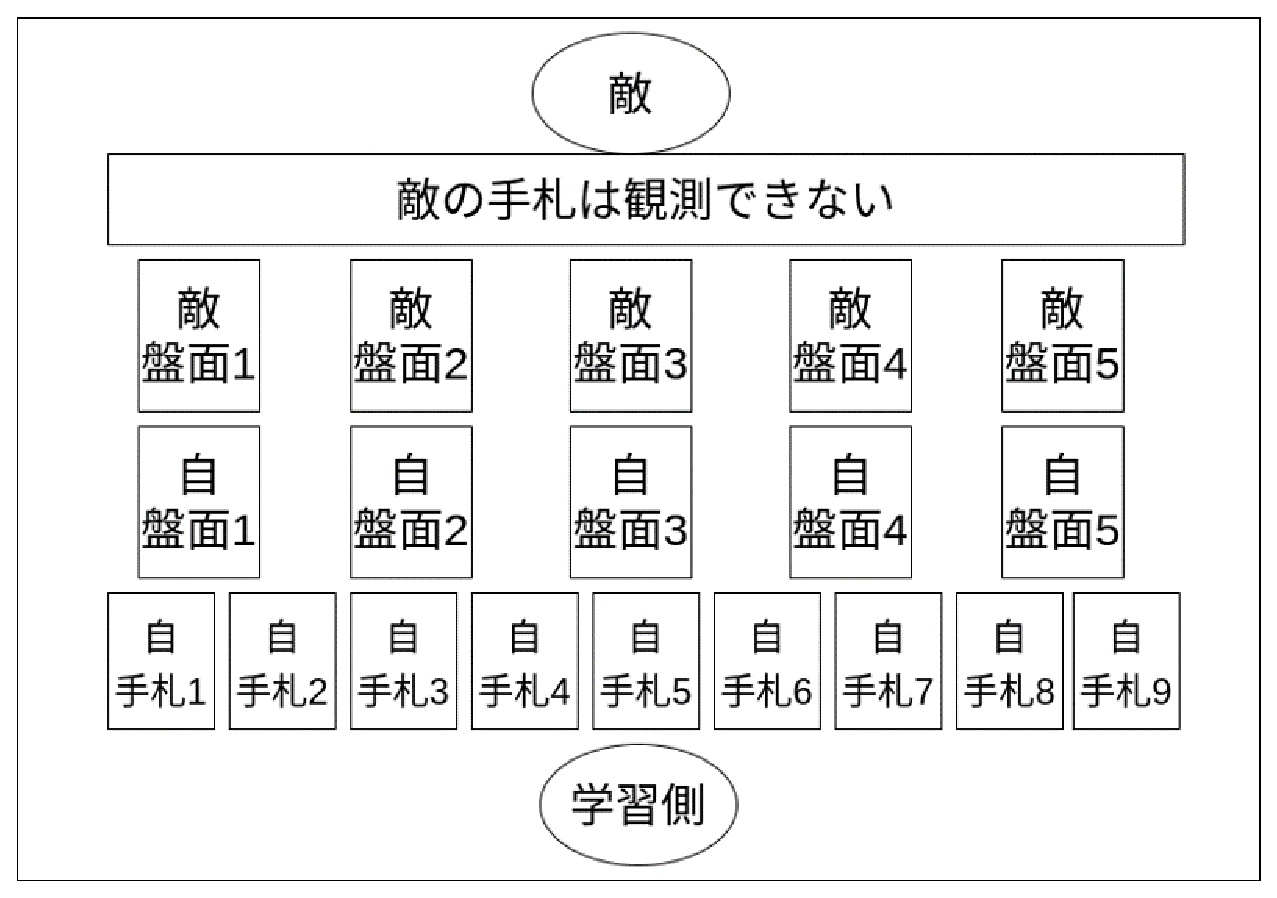
\includegraphics[width=100mm]{assets/cardgameimage.eps}
  \caption{深層強化学習における諸定義イメージ}
  \label{fig:CardGameImage}
\end{figure}

\begin{table}[t]
  \small
  \centering
  \caption{定義した状態空間}
  \label{table:state}
  \vspace{-0.3cm}
  \scalebox{0.90}[0.90]{
    \begin{tabular}{|c|c|c|c|}
      \hline
      状態説明                        & 次元数        & 最小値        & 最大値         \\ \hline \hline
      各プレイヤーの HP & 2 & 0 & 20 \\ \hline
      各プレイヤーの マナ & 2 & 0 & 5 \\ \hline
      \begin{tabular}{c}
        手札 1 $\sim$ 9 の\\HP , 攻撃力, コスト, 特殊効果
        \end{tabular}      & 36         & 0          & 5          \\
      \hline
      \begin{tabular}{c}
        自盤面 1 $\sim$ 5 の\\HP と攻撃力
      \end{tabular}     & 10         & 0          & 5 \\
      \hline
      \begin{tabular}{c}
        敵盤面 1 $\sim$ 5 の\\HP と攻撃力
      \end{tabular}     & 10         & 0          & 5 \\
      \hline
      \begin{tabular}{c}
        自盤面 1 $\sim$ 5 が\\攻撃可能かどうか
      \end{tabular} & 5          & 0          & 1  \\
      \hline
      \begin{tabular}{c}
        お互いのデッキの\\残り枚数
      \end{tabular}     & 2 & 0 & 30 \\
       \hline
      \end{tabular}
  }
  \end{table}

  \begin{table}[t]
    \centering
    \caption{定義した行動空間}
    \vspace{-0.3cm}
    \label{table:action}
    \scalebox{0.90}[0.90]{
      \begin{tabular}{|c|c|}
        \hline
        行動説明                          & 次元数        \\ \hline \hline
        手札 1 $\sim$ 9 を自盤面に出す             & 9          \\ \hline
        自盤面 1 が敵盤面 1 $\sim$ 5 に攻撃or敵プレイヤーに攻撃    & 6          \\ \hline
        自盤面 2 が敵盤面 1 $\sim$ 5 に攻撃or敵プレイヤーに攻撃    & 6          \\ \hline
        自盤面 3 が敵盤面 1 $\sim$ 5 に攻撃or敵プレイヤーに攻撃    & 6          \\ \hline
        自盤面 4 が敵盤面 1 $\sim$ 5 に攻撃or敵プレイヤーに攻撃    & 6          \\ \hline
        自盤面 5 が敵盤面 1 $\sim$ 5 に攻撃or敵プレイヤーに攻撃    & 6          \\ \hline
        ターンエンド & 1 \\ \hline
        \end{tabular}
    }
      \end{table}

\subsubsection{DQN}

\subsection{実験 2 : }

\clearpage
\section{結果と考察}



\clearpage
\newpage
\changeindent{0cm}
\section{まとめと今後の課題}

本研究では, 3 つの手法を提案し, 数値実験用の独自の TCG 環境下で数値実験し提案手法の有効性を検証した.
\par
実験 1 では DQN を用いて人力で構築した戦略よりも高い勝率を記録するエージェントを構築した. また, DQN により構築したエージェントはデッキにおいて人間から見ても妥当な戦略を構築しており, 構築戦略下におけるカードの強弱も学習していることが分かった.
\par
実験 2 では提案手法 2 の数値実験をした. 人力で構築した戦略と DQN で構築した戦略では結果に差があった. DQN ではカードの強弱を学習しているためより人間のプレイに近い結果を得られるといえる.
\par
実験 3 では実験 2 で得られた結果を利用して提案手法 3 の数値実験をした. 調整するカード枚数を増やして GA の解空間の次元を増やすほど勝率に関する適応度は高くなっていた. 
また, 提案手法により得られた解は $f_w$ に関しては多目的 GA により得られた解に優越し, $f_c$ については最も優越する解が得られ, 提案手法の有効性が確かめられた.\par
今後の課題を以下に列挙する.
\begin{itemize}
  \item DQN 以外の深層強化学習手法の適用
  \par
  本研究ではエージェント構築の部分に DQN を適用した. 近年では, DQN に様々な工夫を加えた Rainbow \cite{Rainbow}, ターン制完全情報ゲームで顕著な成果を残している AlphaZero \cite{AlphaZero}, その他にも DreamerV2  \cite{DreamerV2}, MuZero \cite{MuZero}, RebeL \cite{ReBeL} など様々な優れた深層強化手法が提案されている. これらの手法を用いることで DQN と比べてより良い戦略を持つエージェントを構築することが期待できる.
  \item GA 以外の最適化手法の適用\par
  本研究では, ゲームバランスの調整においてデッキ内のカードのパラメータを対象として GA を適用した. GA には初期収束という問題がある. GA の選択ルールに熱力学的
  なエントロピーと温度の概念を取り入れることでこれを解決する TDGA \cite{TDGA} を用いることで提案手法 3 においてより良い解が得られると期待できる.
  \newpage
  \item ハイパーパラメータの最適化
  \par
  本研究では, DQN や GA といったアルゴリズムのハイパーパラメータを人力で設定した. Optuna \cite{Optuna} といったハイパーパラメータのチューニングツールを用いて本研究のタスクに適したハイパーパラメータを見つけることでより良い結果を得ることが期待できる.
  \item デッキ間の相性を考慮したゲームバランス調整方法の検討
  \par
  現在はデッキ間の勝率がどの対戦においても勝率が 50 \% に近いほうがゲームバランスとして良い状態としているが, 実際はデッキ間の相性があり, それを事前に推測するメタゲームという概念がある. このような相性まで考慮したバランス調整が重要である.
\end{itemize}




\changeindent{2cm}

%謝辞
\clearpage
\newpage
\changeindent{0cm}
\acknowledgements
\changeindent{2cm}

\begin{flushright}
  年  月  日
\end{flushright}

% 参考文献
\clearpage
\newpage
% \changeindent{0cm}
% \begin{thebibliography}{99}
%  \changeindent{2cm}
%  \bibitem{taro} らてふ太郎, 『LaTeX入門』 https://medemanabu.net/latex/
% \end{thebibliography}


\bibliography{index}
 \changeindent{2cm}
% \bibliography{index}
\bibliographystyle{junsrt} %参考文献出力スタイル


\end{document}